% Template PNSAC newsletter - Article
% Language: Latex
%

% Head

\title{Conservator's Corner}
%\subtitle{PNS 2016 Status Update}
\author{Bruce Gemmill, R\'{e}jean Demers, and Garry Dupont}
%\author{Restoration Project Manager}

\maketitle

%\section{Zen and the Art of Aircraft Restoration.}

The past year was a very busy one for the North Star restoration crew. 
In the Engine Shop, under the careful watch of Crew Chief Garry Dupont,
members Charles Baril and Richard Lodge worked to fit the final pieces
on engine 4 including; all the cowl frames and panels, main and
auxiliary radiator flaps under the engine, the engine air intake duct
and associated actuators. All the hard work in setting up sheet metal
repairs to the cowl panels paid off.  However, fitting the large steel
exhaust panels around the 12 exhaust stacks was particularly
challenging. It's no longer a secret that ratchet straps and wooden
2"x4" blocks have become part of the standard North Star tool kit.

While that work was underway, Jacques Roy, Peter Scartozzi and Charles
Baril were busy stripping equipment, pipes, hose and cables from inside
the nacelle where engine 4 will soon be installed.  Will Assad and Neil
Raynor also helped with this. After equipment removal, many hours were
spent carefully cleaning and removing oil and corrosion prior to
painting.  In some areas a small bead blasting gun was used to remove
rust from nuts and bolt heads that could not be taken out for cleaning.

Most notably were efforts by Charles Baril, who spent many months
inside the nacelle; cleaning, inspecting and masking off for painting.
The work took so long that special heating ducts and insulation needed
to be positioned around the nacelle to keep it warm enough for R\'{e}jean
Demers and Bruce Gemmill to apply a coat of primer and silver paint.

\begin{figure}[httb]
   \vspace{2em}
   \centering
   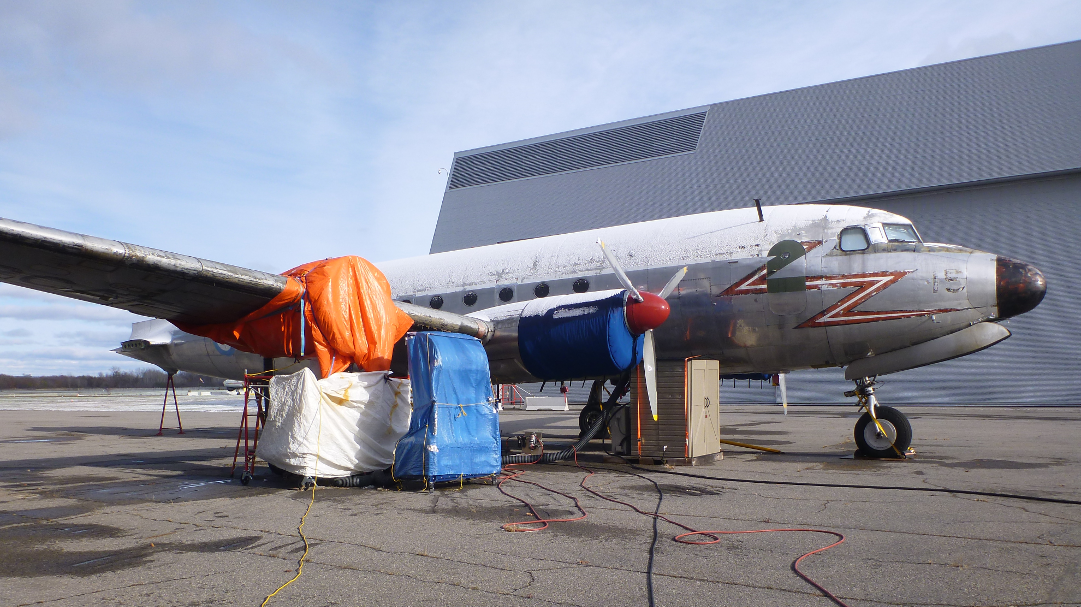
\includegraphics [scale=0.5]{nacelle-4-paining-outside-feb-2020.png}
   \caption*{\small \em Painting nacelle \#4 outside}
   \label{fig:wall-two}
\end{figure}

Soon after the paint was
applied, the North Star was moved inside for the winter. This occurred
November 8th, just 3 days before our first snow storm of the winter.

While all that work was underway, the Airframe Crew was busy on the
structures work.  Peter Trobridge, Michel Cote and Robert Desjardins
fabricated and installed several replacement parts for main cabin
airframe assemblies that had suffered from years of corrosion.  The
crew accomplished a complete review of necessary repairs from front to
back of the main cabin. A hole was patched near the door to the crew
area, at forward bulkhead (station) 301. This offered Chris McGuffin an
intro to sheet metal repairs. Similar corrosion damage around the
windows required parts shaped on wooden jigs made in the shop. Through
careful planning and creative solutions, repairs were completed at STA:
360, and 381. New repairs carried out at starboard STA: 460, 480, 501,
541, 560, 621 and currently, floor repairs in the loading area near the
cargo doors.

\begin{figure}[httb]
   \vspace{2em}
   \centering
   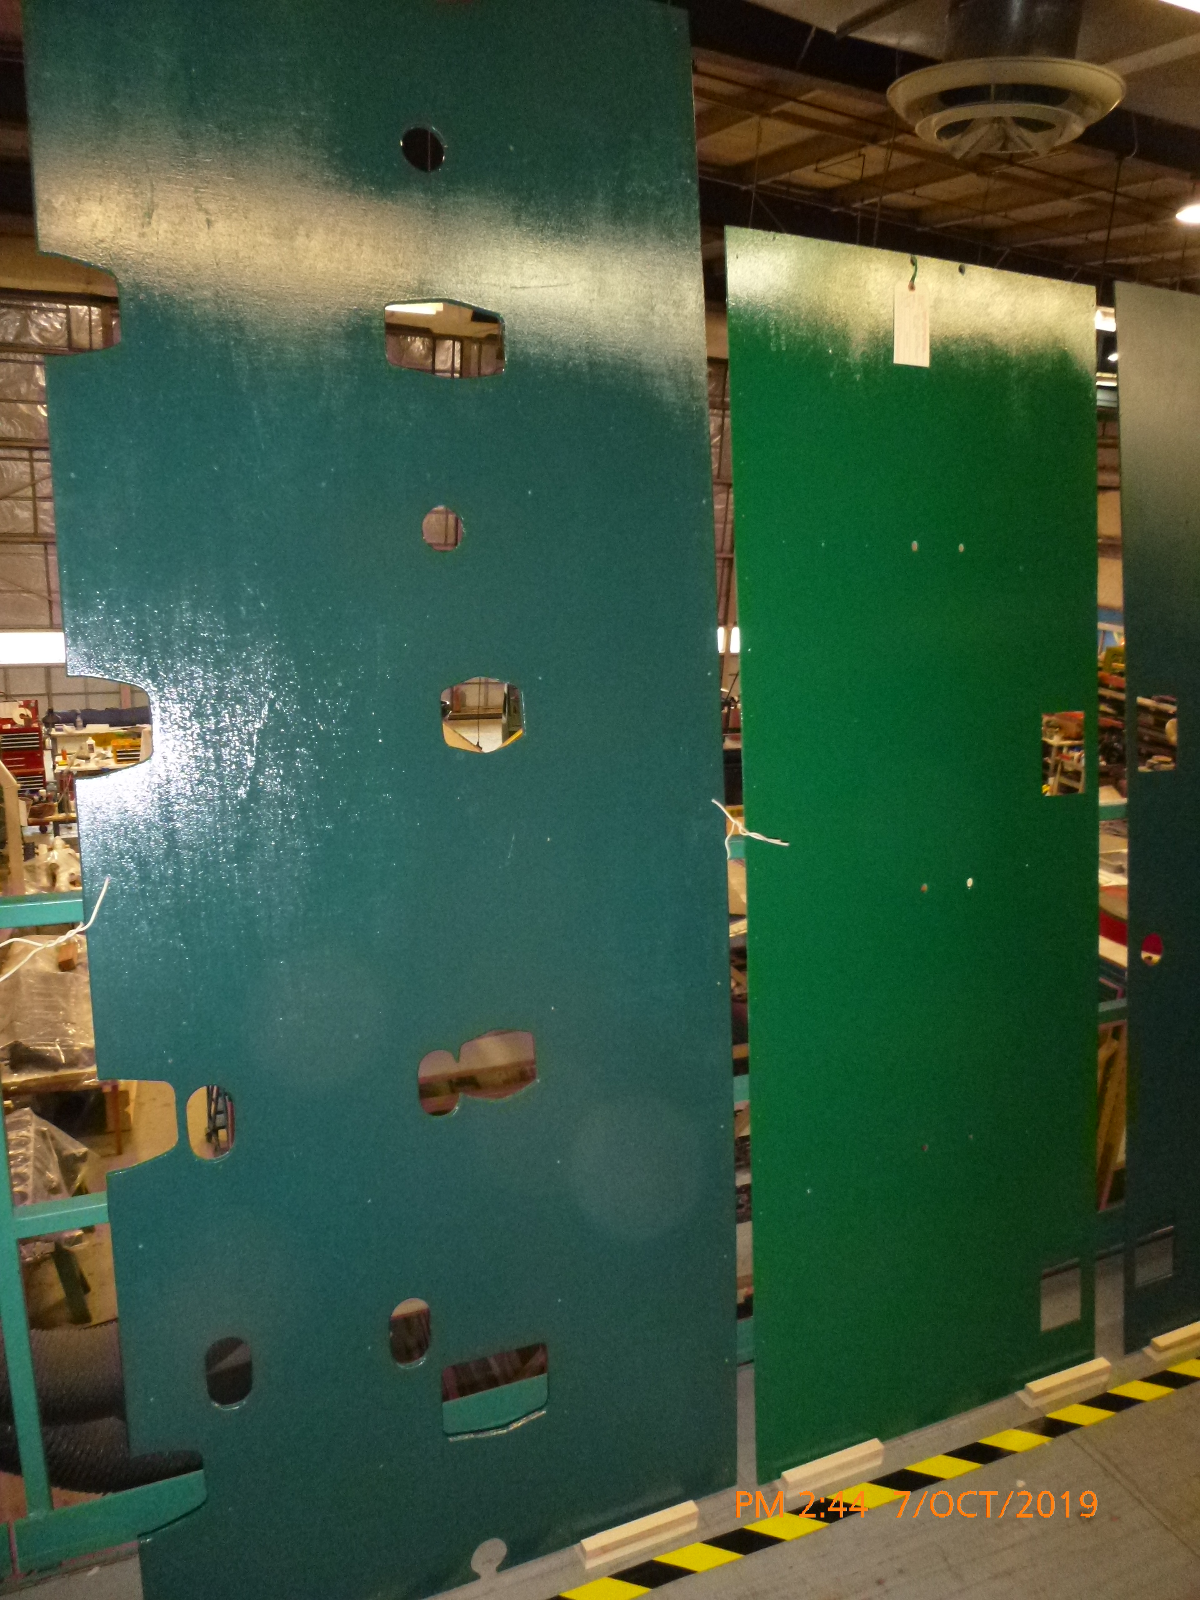
\includegraphics [scale=0.5]{New-Floor-Wall-Panels-feb-2020.png}
   \caption*{\small \em New floor and wall panels}
   \label{fig:wall-two}
\end{figure}

The Carpentry Crew, led by Chris McGuffin measured, cut and trimmed new
plywood panels for the interior walls of the main cabin.  These were
painted green to match the original colour scheme, then set aside until
for later installation.  Next came the floor panels.  Richard Houle and
John Makadi assessed these, according to the amount of damage caused by
wear and tear, as well as leaks around windows and doors.  Some panels
were salvaged with a few minor repairs, then painted. These are now
ready for installation.  Several others were so badly damaged that
completely new panels needed to be made. 

Finally, work started on the third group of panels.  These floor panels
had significant damage to one or two edges.  The damaged areas need to
be cut away and a new piece added by bevelling the adjoining pieces
using what is called a "scarf joint" so the adhesive bond is strong.  A
special jig was constructed to do this work, allowing an electric
router to run at an angle to produce the joint. A Resorcinol
Formaldehyde adhesive will assure a long-lasting repair.

Many of the volunteers got to work on the large collection of
accessories that had been removed from nacelle \#4.  This included
pumps, plumbing, fluid and air lines, control cables, bell cranks and
pulleys, electrical harnesses, valves and filter canisters. Each needed
assessment, cleaning, repair, polishing or painting as well as
documentation and photographs of the work undertaken. Phil Chrysler and 
Brian Cole went to work on the many fairings and
access panels that also required cleaning and polishing to be ready to
be placed back on the aircraft. A special mention should be made for the late
Ted Devey who had had his hand on a few cowl panels and nacelle components.

Several special projects were also undertaken during the year.  John
Makadi removed the nose radome to determine what radar equipment had
been removed, in case we are able to find a source for missing
equipment.  We removed the upper rotating navigation beacon to fix a
persistent leak, this necessitated a twin tower scaffold assembly to
safely reach the top of the fuselage. Neil Raynor and Will Assad
overhauled a propeller stand the Museum had not used for many years. 
It got a fresh coat of paint and new wheels and tires, and is now
holding two North Star propellers, until they can be installed on the
appropriate engine. 

\begin{figure}[httb]
   \vspace{2em}
   \centering
   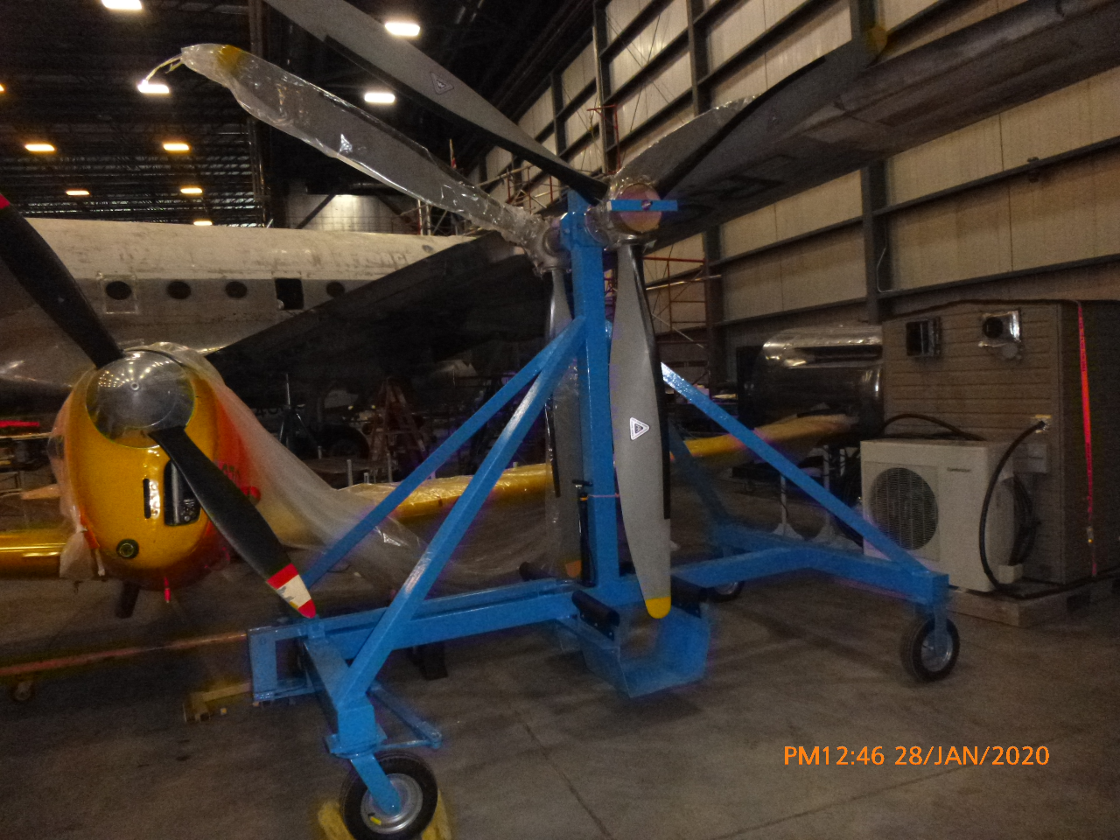
\includegraphics [scale=0.5]{prop-stand.png}
   \caption*{\small \em Prop stand}
   \label{fig:wall-two}
\end{figure}

Michael Hope
assisted in removal of Prop. \#1 and assembly of soon-to-be-installed
Prop. \#4. Phil Chrysler and Brian Cole fabricated cables and special
fittings to secure the landing gear so the aircraft could be safely
displayed. Other duties  such as; an inventory of replaced / restored
and spare components were carried out.  All of these were packed and
stored in a new location of the Reserve Hangar.

\begin{figure}[httb]
   \vspace{2em}
   \centering
   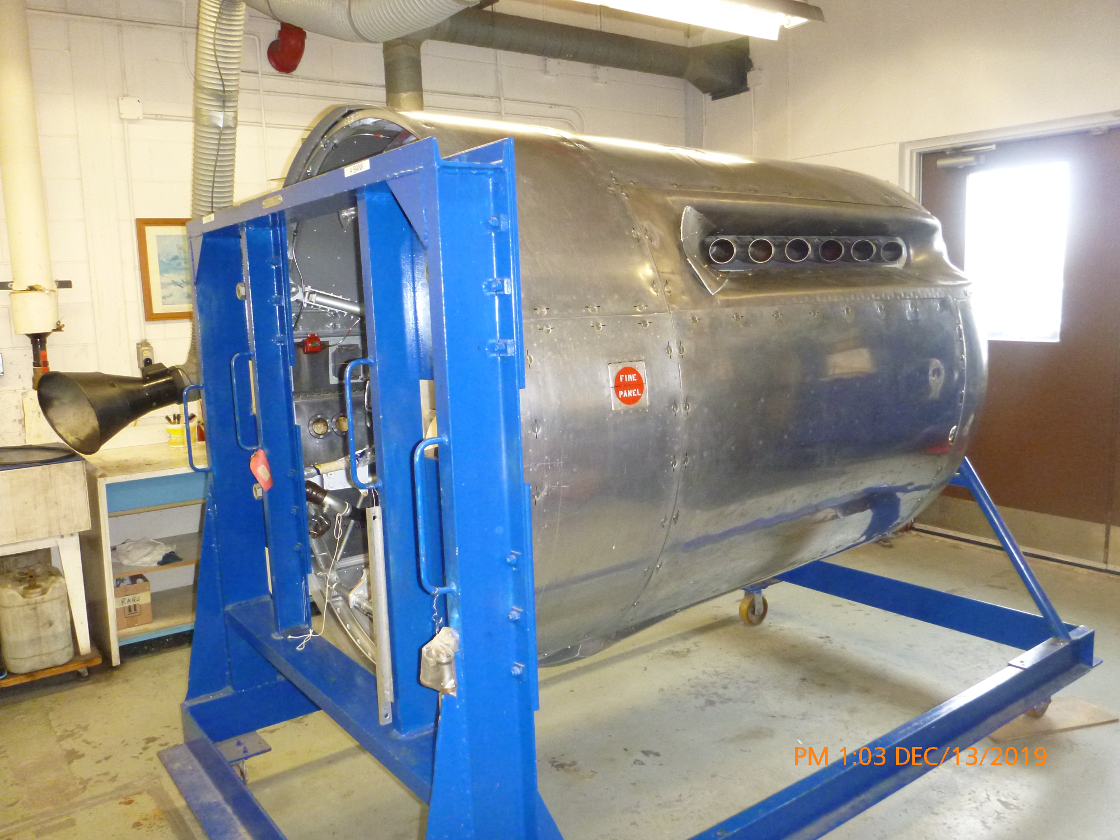
\includegraphics [scale=0.5]{eng-4-pre-move-feb-2020.png}
   \caption*{\small \em Engine \#4---before it was moved to the Reserve Hangar}
   \label{fig:wall-two}
\end{figure}

Number \#4 engine has now  been moved to the Reserve Hangar. The crew
are prepping the oil tank for clear coat then it will be assembled and
ready to install. Once this is completed  the plan is to carry out some
deep cleaning and renovations in the shop starting  by  relocating the
varsol cleaning tank. The paint shaker has been repaired and the base
has been painted ready for assembly. The paint shaker will be relocated
where the varsol tank was. The old roll away tool box has been replaced
by a new Snap-On unit. There have been lots of comments on the orange
colour  but the price was right.

Currently, work is on-going to complete the rear (main) cargo door and
quilted liner installation. Nacelle \#4 installation of restored
components is advancing in small steps, due to the complexity of
interrelated systems and locations. Scaffolding is in place, over the
forward fuselage area above the cockpit to assess air-frame
requirements and treatment methods to be used on exterior hull
surfaces. Restoration records are also being reviewed by Conservation
Special Project Manager R\'{e}jean Demers. The Work Order / Task Card
format is lending well to Museum information uploading tools. Efforts
are underway to recruit two to four new shop volunteers, and R\'{e}j
invites any new applicants referred by PNSAC to apply.

\begin{footnotesize}
  \raggedleft PNSAC\\
\end{footnotesize}

% End of text.

%%% Local Variables: 
%%% mode: latex
%%% TeX-master: main_document.tex
%%% End: 

